\section{Repository state as an executable environment}\label{sec:C23:repository}
A repository task is a partially observed transition problem. The agent observes selected files, search results, test outputs, and version-control metadata. It acts through edits, commands, dependency operations, and sometimes remote services. The true environment includes build tools, generated files, network dependencies, and hidden tests that may not appear in its initial context. Treating the task as text completion discards the execution feedback that makes repository-level work distinctive.

The action interface should preserve artifact identity. A patch request names its base revision and intended file changes; command execution records working directory, environment, exit status, and captured output. The test verdict binds to the resulting artifact digest. If the agent edits code after testing, the verdict must be invalidated or rerun. This mechanical correspondence is separate from whether the tests capture the intended behavior.

An execution attestation can make that boundary explicit. Let $A$ be the tested artifact, $D$ its declared dependency/environment manifest, and $e=(a,d,q,x,\tau)$ record their digests, the exact test invocation $q$, exit status $x$, and execution trace $\tau$. With $\kappa(\tau)=1$ denoting a complete, attributable invocation record, define
\begin{equation}
 v_e(A,D)=\mathbf1\{a=h(A)\}\mathbf1\{d=h(D)\}
          \mathbf1\{x=0\}\mathbf1\{\kappa(\tau)=1\}.
 \label{eq:C23:artifact_attestation}
\end{equation}
This predicate establishes provenance of a zero-exit execution for the declared inputs, assuming collision-resistant hashing and trustworthy records. It does not establish requirement coverage, authentic dependencies beyond the captured manifest, or absence of unrecorded network/environment changes. A failed command followed by a persuasive final message has $v_e=0$; an edit after testing changes $h(A)$ and invalidates the old attestation. Test discovery failures and a command that executes no relevant tests still require separate validation even when its exit status is zero.

The 2024 SWE-agent study established an influential interface baseline and demonstrates the importance of the agent-computer interface rather than model capability alone~\cite{yang2024sweagent}. Search, file navigation, editing, and error feedback change how effectively the model can act on repository state. The proper inference is interface sensitivity in the studied setting. It does not establish that one interface dominates across languages, repositories, models, and tool latency. A useful replication preserves the evaluator and workload while varying only the interaction surface.

The implementation anchor is an actual rollout through the published repository: model input construction, command interface, environment stepping, output truncation, and termination. A researcher should locate the callable that executes actions and the adapter that converts its results back into model-visible messages. Silent truncation or error normalization can materially change the policy. Comparing only prompt templates misses those mechanisms.

Repository isolation also matters. An agent should not see another benchmark task's generated artifacts or hidden test outcomes through a shared checkout or cache. The workspace, dependencies, and stateful tools need a reset policy. Reusing a build cache may be legitimate for cost analysis but must not transfer answer-bearing files across tasks. Separate a warm infrastructure cache from persistent semantic memory and report both explicitly.



Figure~\ref{fig:C23:overview} isolates the mechanism and its stated information boundaries.
\begin{figure}[!htbp]
\centering
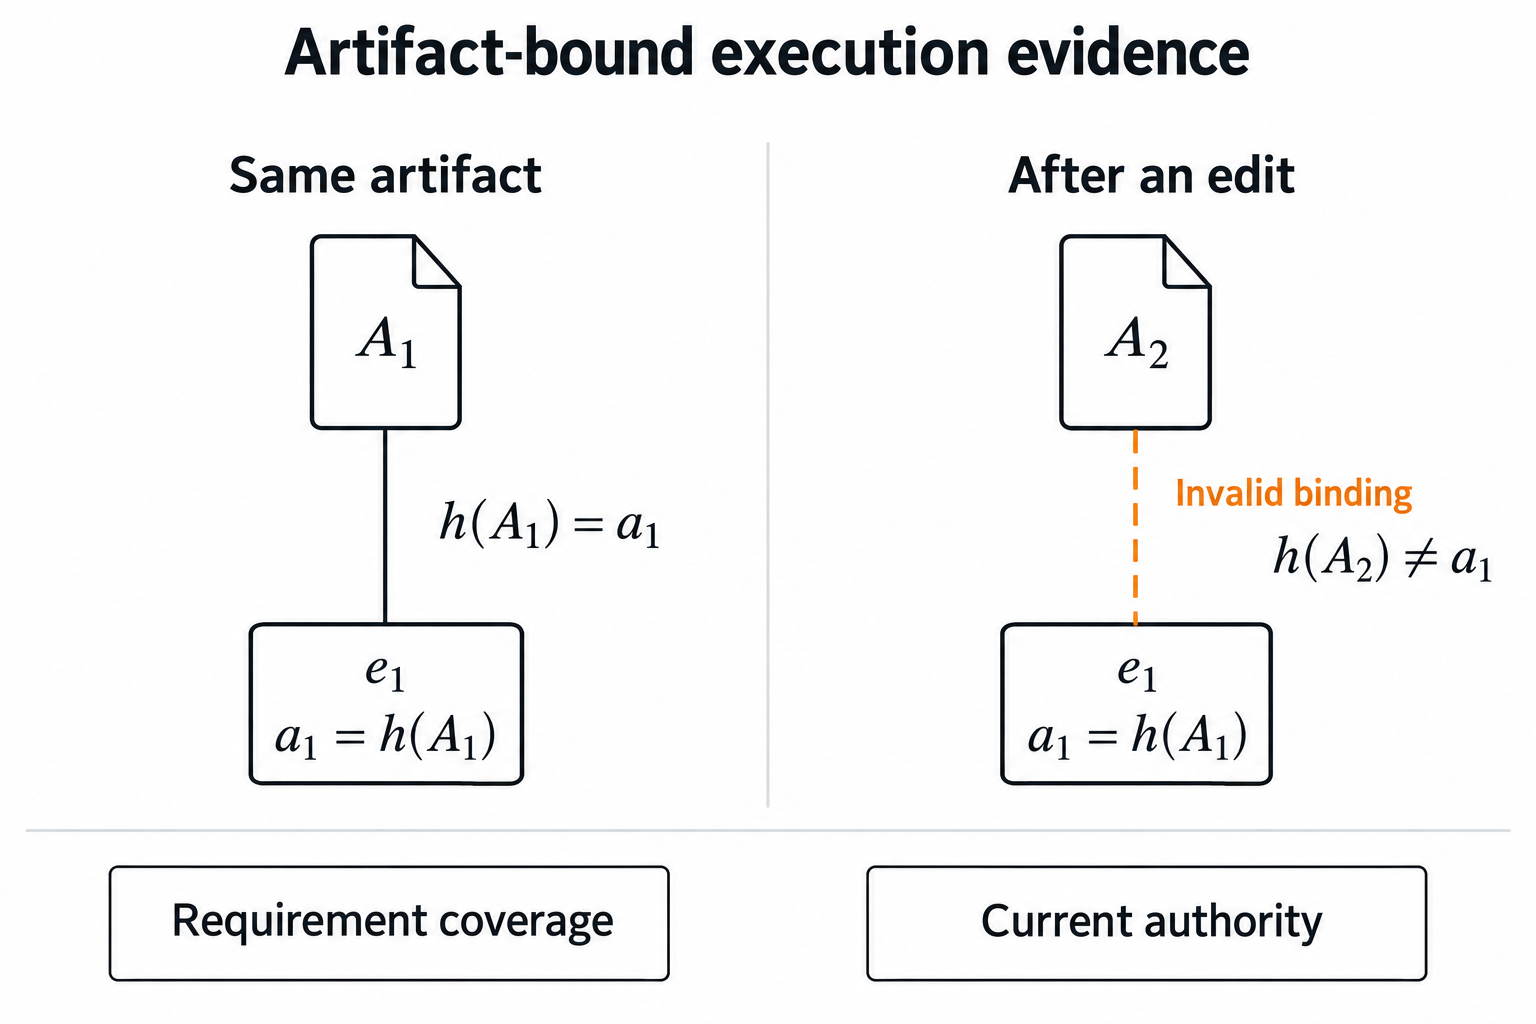
\includegraphics[width=\linewidth]{book/figures/assets/F23review.png}
\caption{The same execution record is checked against two artifact revisions. It binds to the tested artifact in the left panel; the illustrated edit changes the digest and invalidates that binding in the right panel. Matching provenance identifies the object tested, while requirement coverage, the declared environment and current authority need their own checks.}
\label{fig:C23:overview}
\end{figure}
